\subsection{Автоматическая проверка произношения}

\subsubsection{Введение}
Роль IT-технологий в изучении иностранных языков с течением времени лишь увеличивается. Изначально программные средства были достаточно просты и использовали лишь текст со статическими изображениями для подачи материала, а для взаимодействия с пользователем в основном использовался письменный ввод. С развитием технологий машинного обучения стало возможным значительно расширить способы передачи информации между пользователем и обучающей системой. Так, в данной работе рассматривается задача анализа голосовой речи студента на иностранном языке для выявления ошибок и подсказок по их исправлению. Программа должна уметь давать обратную связь, схожую на ту, которую дал бы преподаватель, оценить качество произношения в целом и указать на конкретные ошибки студента.

Эта задача принадлежит к области автоматического распознавания речи (ASR), однако стандартные ASR алгоритмы не приспособлены для задачи оценки произношения и поиска ошибок. По этой причине возникает необходимость создания новых, более узконаправленных решений поставленной задачи.

Существуют различные подходы к оценке качества произношения, некоторые из них производят оценку предложения целиком, другие -- отдельных слов, мы же будем рассматривать систему, позволяющую проводить оценку речи на иностранном языке на уровне фонем. Этот подход позволяет обнаруживать ошибки произношения в конкретных звуках и выявить разницу между эталонным звучанием и произношением студента.

\subsubsection{Особенности обучения фонетике иностранных языков}
В данной работе рассматриваются способы тренировки устной иностранной речи. Использование компьютерных средств обучения несет в себе ряд преимуществ. В отличие от занятий в классе, где учителю приходится прерываться и распределять внимание на всех студентов, при таком подходе ученик может заниматься непрерывно. Помимо этого, на занятиях в группах некоторые ученики чувствуют себя скованно и постоянно сравнивают себя с другими. К тому же программа является бесконечно терпеливой и позволяет потратить столько времени на изучение темы, сколько необходимо.

Конечно, у автоматизации процесса обучения есть и свои недостатки. Так, грамотный преподаватель как правило насыщает урока разнообразными учебными активностями и мотивирует студентов развиваться. Кроме социальной стороны, есть и определенные технические ограничения в распознавании речи и анализе ошибок произношения.

Перед построением и применением алгоритмов машинного обучения при оценке произношения и анализе ошибок необходимо сначала разобраться в фундаментальных аспектах обучения иностранной речи.

Что мы рассматриваем в качестве <<правильного>> произношения? Конечно, нельзя строго определить единый вариант <<правильного>> произношения -- во многих языках есть диалекты, а иногда даже в одном диалекте есть несколько корректных вариантов произношения одного слова. Тем не менее, мы можем объективно оценить ключевые характеристики речи:
\begin{itemize}
	\item произношение отдельных фонем;
	\item произношение фонем вместе с другими, в контексте слов и предложений;
	\item интонация;
	\item тон и ритм речи;
	\item ударение.
\end{itemize}
В данной работе мы по большей части сосредотачиваемся на характеристиках произношения отдельных фонем и их звучания в контексте других фонем.

Своей целью в рамках этого раздела мы ставим создание инструмента, который позволит пользователю изучать правильный вариант произношения, выполнять проверку своей устной речи и получать в ответ анализ ошибок. Как было установлено ранее \cite{rogers1994intelligibility}, использование программных средств действительно способно улучшить произношение иностранных слов. А первые способы автоматической оценки устной речи были представлены еще в 1995 году \cite{anderson1995evaluation}.

\subsubsection{Алгоритмы машинного обучения для автоматической проверки произношения}
В предыдущих пунктах мы определили основные характеристики речи, на которые нужно обратить внимание и выяснили особенности обучения произношению иностранных слов. Теперь рассмотрим как с помощью этой информации мы можем построить систему автоматического анализа устной речи.

В целом обучающая система должна выполнять задачи, которые ставятся перед преподавателем языка. В дополнение к этому система может содержать те методы обучения, которые было бы затруднительно реализовать при обучении с учителем. Алгоритмы автоматического распознавания речи предоставляют мощный набор инструментов для работы с устной речью студента. Тем не менее, для использования в этом контексте их необходимо модифицировать и улучшить в следующих аспектах:
\begin{itemize}
	\item распознавание речи, содержащей ошибки и сильный акцент;
	\item внедрение возможности оценки правильности произношения;
	\item разработка функции обнаружения и анализа ошибок;
\end{itemize}

Для повышения эффективности распознавания искаженной речи необходимы значительные изменения в работе акустических моделей. Так, в предыдущих работах демонстрировалось\cite{ehsani1997subarashii}, что переобучение моделей на речи не носителей языка, содержащей ошибки, позволяет значительно повысить качество распознавания. Тем не менее, такой подход требует больших объемов данных с речью не носителей языка, что не всегда доступно или возможно. В других работах\cite{thelen1997speaker} представлены методы обобщения моделей с использованием метода максимального правдоподобия в линейной регрессии, что позволяет значительно снизить объем необходимых данных.

В последние годы было представлено несколько подходов к оценке правильности произношения. Так, в одном из первых таких подходов\cite{hamada1993automatic}, оценка производится путем вычисления разницы спектров аудио с записью речи студента и эталонным вариантом произношения, используя векторное квантование\footnote{Квантование -- методика, при которой множество с большим количеством элементов приводится к множеству с меньшим (счетным) количеством элементов путем разделения на группы с приблизительно схожими свойствами и взятием из каждой группы одного элемента-представителя.} и динамическую трансформацию временной шкалы.

Другие подходы\cite{neumeyer1996automatic,franco1997automatic} направлены на оценку более длинных фрагментов речи, например, предложений, с использованием принципа апостериорного максимума\cite{wiki:Maximum_a_posteriori_estimation}. Такой метод оценки речи имеет высокую корреляцию с оценками, которые выставляют эксперты, однако имеет существенный недостаток в том, что оценка всего предложения сама по себе не даёт информации для проведения анализа ошибок.

Для решения этой проблемы применяется оценка речи на уровне фонем с использованием вероятностных моделей \cite{kim1997automatic}. Использование алгоритма, основанного на логарифме апостериорной вероятности позволяет достигать корреляции $r_{xy}=0.72$ между оценками системы и оценками экспертов.

В данной работе мы остановимся на методах, которые позволяют достичь наилучших результатов -- вероятностные модели с использованием скрытых Марковских моделей, а также продемонстрируем использование глубоких нейронных сетей для моделирования вероятностей переходов состояний в скрытых Марковских моделях. В последующих пунктах мы подробнее рассмотрим эти алгоритмы.

\subsubsection{Скрытые Марковские модели в распознавании речи}
Система автоматического распознавания речи состоит из нескольких этапов. Сначала звуковой сигнал преобразовывается в набор векторов признаков. Затем векторы подаются на вход сети-декодеру, который состоит из скрытой Марковской модели, языковой модели и словаря. На заключительном этапе наиболее вероятный путь через сеть определяет наиболее вероятную последовательность слов для входного звукового сигнала.

Общая структура работы такого процесса изображена на рисунке \ref{fig:asr-architecture}.
\begin{figure}[h]
	\centering
	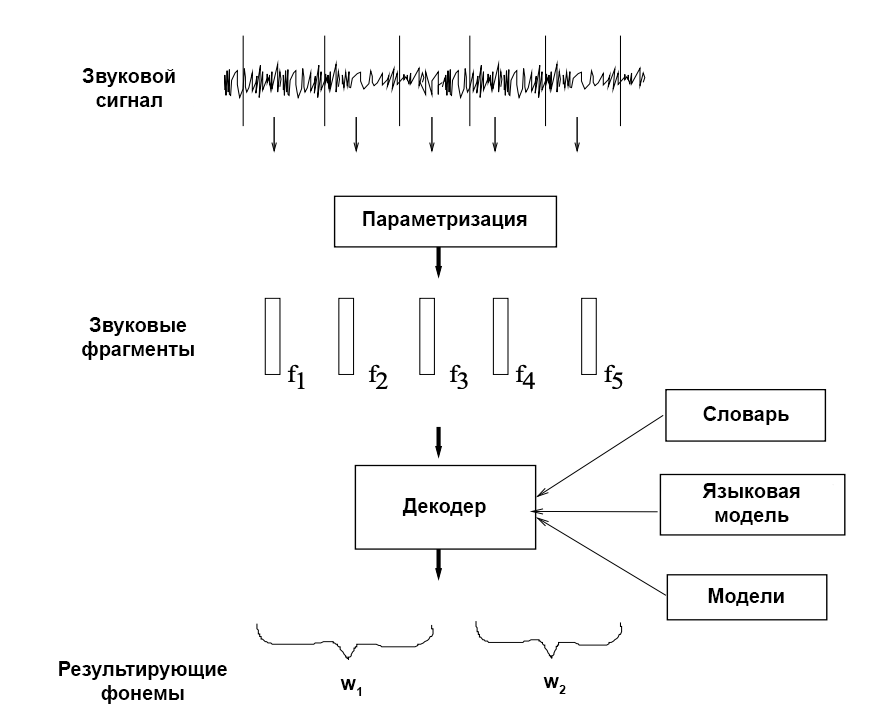
\includegraphics[width=0.7\textwidth]{asr-network-structure}
	\caption{Структура системы автоматического распознавания речи.}
	\label{fig:asr-architecture}
\end{figure}

На самом первом этапе в системе распознавания речи необходимо семплировать входящий аналоговый аудиосигнал с частотой как минимум в два раза превышающей максимальную частоту, содержащуюся во входном сигнале \cite{wiki:Nyquist-Shannon_sampling_theorem, web:music_and_computers_sampling}.

Далее оцифрованный аудио сигнал разбивается на 16-битные фрагменты, называемые кадрами. Такие кадры как правило длятся в пределах 15-20 миллисекунд.

Каждый кадр проходит этап параметризации. Параметризация речи направлена на извлечение ограниченного набора характеристик речи, которые не зависят от автора звукового фрагмента, записывающего оборудования и других несущественных факторов. Затем полученные параметры речи подаются на вход последующим этапам обработки речи. Детали процесса параметризации речи приводятся в источнике\cite{ganchev2011contemporary}.

Скрытые марковские модели широко применяются в системах распознавания речи. Ниже приводится краткий обзор теории, которая стоит за Марковскими моделями. 

Скрытую Марковскую модель можно рассматривать как конечный автомат, который совершает переход через равные интервалы времени, и обладает следующими параметрами:
\begin{itemize}
	\item Множество скрытых состояний $S = \{S_1, \dots, S_N\}$;
	\item Множество результатов наблюдений;
	\item Матрица вероятностей перехода $A = [a_{ij}]$, где $a_{ij}$ -- вероятность перехода из состояния $i$ в состояние $j$
	$$ a_{ij} = p(s_{t+1}=j|s_t=i)$$
	\item Вероятности нахождения автомата в каждом из состояний в начальный момент времени;
	\item Функция плотности вероятности, определяющая вероятность выпадения каждого из наблюдений при заданном скрытом состоянии. Функция плотности вероятности $b_i(\textbf{o}_t)$ может быть как обычным нормальным распределением, так и смесью $M$ гауссовских распределений. Так, если автомат находится в состоянии $i$, то вероятность наблюдения факта $b_i$ для заданного вектора кадра аудио сигнала $\textbf{o}$ вычисляется по формуле
	$$b_i(\textbf{o}_t) = \sum_{k=1}^{M}w_{ik}b_{ik}(\textbf{o}_t)$$
	Функцию плотности вероятности получим из формулы нормального распределения:
	$$b_{ik}(\textbf{o}_t) = \frac{1}{(2\pi)^\frac{n}{2} \left| C_{ik} \right|^\frac{1}{2}} \exp\left(-\frac{1}{2}\left(\textbf{o}_t - \mu_{ik}\right)' C^{-1}_{ik} \left(\textbf{o}_t - \mu_{ik}\right)\right)$$
	Здесь $\mu_{ik}$ -- среднее компоненты $k$ (вектор длины $n$), $w_{ik}$ -- вес смеси, $C_{ik}$ -- ковариационная матрица размером $n \times n$.
\end{itemize}

Каждая фонема языка может быть представлена скрытой марковской моделью с начальным, конечным и тремя скрытыми состояниями и одной гауссовской смесью для каждого из состояний.

Оценка параметров скрытых марковских моделей производится на больших объемах данных, для которых результат распознавания заведомо известен. Одним из известных методов нахождения вероятностей переходов и параметров функции плотности вероятности является метод максимального правдоподобия\cite[с.~342]{rabiner1993fundamentals}. Ставится задача нахождения набора параметров скрытой марковской модели, на котором функция правдоподобия для данной модели на обучающей выборке принимает максимальное значение (т.е. набор параметров, на которых модель лучше всего <<подходит>> к обучающей выборке). Подбор неизвестных параметров скрытой марковской модели можно реализовать с помощью частного случая EM--алгоритма\cite{dempster1977maximum} --- алгоритма Баума--Велша. Это итеративный алгоритм, направленный на нахождение параметров (вероятности переходов, вероятности наблюдений и изначальное состояние), для которых будет достигаться максимальное значение правдоподобия на обучающей выборке.

После нахождения параметров модели можно приступать к её использованию. Распознавание речи с помощью скрытых марковских моделей основано на нахождении последовательности элементов речи, которые вероятнее всего порождают данный звуковой сигнал в форме последовательности аудио-фрагментов (кадров).

Формально систему распознавания речи можно представить в виде уравнения:
$$\mathbf{\hat{W}} = \operatorname{arg} \max_\mathbf{W} P(\mathbf{W} | \mathbf{O}).$$
Здесь $\mathbf{W} = w_1, w_2, \dots, w_n$ --- это последовательность элементов речи (например, фонем), $\mathbf{O} = \mathbf{o}_1, \mathbf{o}_2, \dots, \mathbf{o}_T$ -- последовательность кадров аудио сигнала.

Сама условная вероятность может быть выражена с использованием формулы Байеса:
$$P(\mathbf{W}|\mathbf{O}) = \frac{P(\mathbf{O}|\mathbf{W})P(\mathbf{W})}{P(\mathbf{O})}.$$

Здесь $P(\mathbf{W})$ обозначает вероятность произнесения последовательности $\mathbf{W}$. Эта вероятность --- языковая модель, не зависящая от входного звукового сигнала и основанная исключительно на предварительных данных. Вероятность $P(\mathbf{O})$ --- это средняя вероятность наблюдения последовательности $\mathbf{O}$.

Построенные модели в своём базовом варианте не предназначены для распознавания искаженной речи. Как правило, речь студентов, которые занимаются изучением иностранного языка, значительно отличается от эталонной. Так, определенный класс фонем может заменяться на другие, более привычные, варианты из родного языка. Иногда могут происходит случайные вставки сторонних фонем или же наоборот пропуски. Сам темп речи на новом для человека языке обычно значительно ниже, содержит паузы и повторы. Эти проблемы усложняют задачу распознавания речи.

На этом мы завершим обзор основных принципов распознавания речи с помощью скрытых марковских моделей. Данный класс моделей широко применяется в задачах ASR ввиду своей простоты, возможности автоматического обучения и относительно низкой стоимости вычислений. Тем не менее в последнее время стали появляться более прогрессивные решения с использованием глубокого обучения, имеющие ряд преимуществ. Об этих подходах пойдёт речь в последующих пунктах.

\subsubsection{Использование CNN в задаче распознавания речи}
Сверточная нейронная сеть -- это алгоритм глубокого обучения, наиболее широко применяющийся для обработки визуальных данных, в рекомендательных системах\cite{cnn-recomendation-system} и при работе с естественным языком\cite{cnn-nlp}. Некоторые аспекты сверточных сетей были вдохновлены зрительной корой мозга животных\cite{cnn-neocognitron}. Предварительная обработка данных, требуемая в сверточных сетях, значительно ниже по сравнению с другими алгоритмами классификации. Для адаптации сверточных сетей к задаче распознавания речи необходимо трансформировать входные данные в так называемые карты признаков --- двухмерное представление поступающего аудио сигнала.

Отличительными особенностями сверточных сетей являются их способность сохранять пространственную структуру входных данных и возможность автоматического обучения признакам/характеристикам, которые присущи конкретному классу объектов. Возможность запоминать и прослеживать пространственные связи во входных данных позволяют достигать высоких результатов в сферах компьютерного зрения и обработки естественного языка, недоступных для классических моделей с многослойным перцептроном и полностью связанных слоев.

\begin{figure}[h]
	\centering
	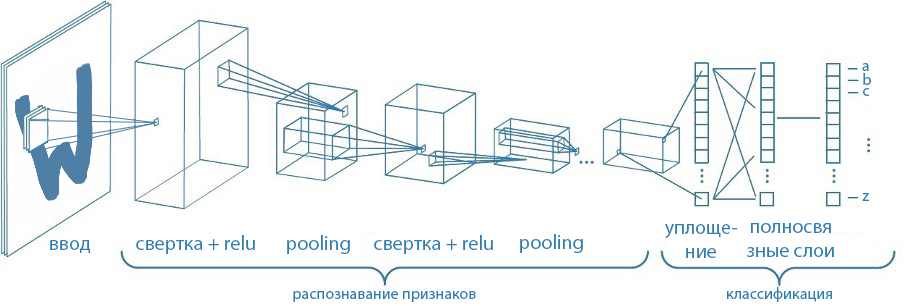
\includegraphics[width=1\textwidth]{cnn-architecture}
	\caption{Архитектура CNN сети.}
	\label{fig:cnn-architecture}
\end{figure}

Классическая сверточная сеть состоит из входного и выходного слоев, а также некоторого количества скрытых, внутренних слоев (Рис. \ref{fig:cnn-architecture}). Внутренние слои сверточной нейронной сети как правило состоят из серии слоёв, производящих \emph{свертку} с использованием ReLU\footnote{ReLU -- англ. Rectified Linear Unit, функция $f(x)=max(0,x)$} в качестве функции активации, после которой следуют остальные слои свертки, чередующиеся со слоями пулинга/субдискретизации. После прохождения нескольких слоев свертки и уплотнения, изначальная карта признаков с высоким разрешением превращается в более абстрактную карту признаков, представляющую высокоуровневые характеристики. В конце эти данные «уплощаются», то есть из тензора преобразуются в вектор и подаются на вход обычной полносвязной нейронной сети, которая тоже может состоять из нескольких слоев. В полносвязной части сети пространственная структура данных утрачивается, размерность в сравнении с исходным изображением значительно падает и основной задачей становится классификация на основе полученной карты признаков. Далее эти приемы будут рассмотрены подробнее.

Отличительной чертой сверточных нейронных сетей является наличие слоев свертки, которые учитывают пространственную структуру изображения. Слои свертки направлены на извлечение ключевых признаков из карты признаков. На вход слоя свертки поступает тензор размерности (ширина карты) $\times$ (высота карты) $\times$ (глубина карты), при обработке используется набор так называемых фильтров, за счет которых и производится свертка. Фильтр представляет собой тензор с тремя измерениями, где глубина совпадает с глубиной входных данных, а размер фильтра выбирается как правило небольшой, например, 3$\times$3 или 5$\times$5.

Операция свертки заключается в следующем. Фильтр с определенным шагом передвигается по всевозможным позициям во входной карте признаков; на каждом шаге вычисляется сумма произведений соответствующих элементов фильтра с текущим рассматриваемым фрагментом входных данных. Эта сумма записывается в выходной тензор.

Таким образом, каждый сверточный нейрон обрабатывает только данные, попадающие в свое «поле зрения». Такой подход позволяет выполнять множество полезных операций: обнаружение краев, размытие или повышение резкости применением различных фильтров.
Шаг движения фильтра – один из гиперпараметров модели. Чаще всего он принимает значения 1 или 2.
Иногда применяется прием добавления отступов к входному тензору для того, чтобы размер исходного тензора совпадал с размером результирующей карты признаков.

\emph{Pooling} слои уменьшают разрешение входного изображения, используя некоторую нелинейную операцию. Так, например, слой \emph{max-pooling} может уменьшить размер изображения вдвое, превращая фрагменты изображения размера 2$\times$2 в одно значение, выбирая максимальный из 4-х пикселей. Наиболее распространенными типами таких слоев являются:
\begin{itemize}
	\item max-pooling;
	\item pooling по среднему значению;
	\item pooling по сумме значений.
\end{itemize}

Типы слоев отличаются функцией, которая применяется к пикселям. Наиболее хорошо на практике показал себя метод \emph{max-pooling} \cite{cnn-max-pooling}. Действие слоя \emph{max-pooling} продемонстрировано на рисунке \ref{fig:max-pooling}.
\begin{figure}[h]
	\centering
	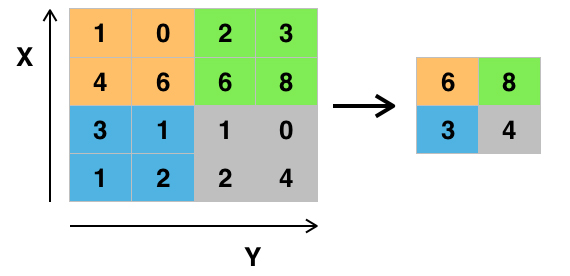
\includegraphics[width=0.7\textwidth]{max-pooling}
	\caption{Пример действия слоя \emph{max-pooling}.}
	\label{fig:max-pooling}
\end{figure}

\emph{ReLU} – функция, определяемая как $f(x)=max(0, x)$. Использование этой функции, по сравнению с другими, повышает нелинейность модели и качество принятия решений без внесения изменений в работу сверточных слоев\cite[с.~3]{cnn-imagenet}. Популярность \emph{ReLU} в качестве активационной функции обусловлена хорошей скоростью обучения моделей.

Введение \emph{dropout}-слоев связано с проблемой переобучения сетей\cite{dnn-dropout}. Суть слоев этого типа в исключении случайных нейронов из рассмотрения при обучении. Это препятствует компонентам сети использовать взаимную адаптацию на данных для обучения, то есть предотвращает «заучивание» данных, на которых тренируется сеть.

После части сети, отвечающей за извлечение признаков, идет несколько полносвязных слоев, которым подается уплощенная карта признаков для проведения классификации. На этом этапе сеть работает с признаками высокого уровня.

В контексте задачи распознавания речи из аудио сигнала необходимо представить входные данные так, чтобы сохранять локальные характеристики относительно частоты и времени. Сохранение характеристик относительно времени не представляет проблемы: в каждый фрагмент входных данных для CNN можно включить 10--15 звуковых фрагментов (кадров) и обеспечивать достаточно контекста. Что касается частоты, то здесь можно использовать линейный спектр или мел--спектр\footnote{Мел--спектр --- спектрограмма, построенная на основе единицы высоты звука мел. Мел получается из герц по формуле $m = 1127 \ln \left(1 + \frac{f}{700}\right)$. Удобство такой шкалы связано с тем, что изменение частоты в герцах воспринимается человеком нелинейно --- разница в 100 Гц между низкими частотами ощущается сильнее, чем между высокими. Мел позволяют выравнять такое расхождение.}, которые сохраняют локальность.

Исходя из этого, входной тензор будет состоять из нескольких звуковых кадров, склеенных между собой и представленных в виде линейного или мел--спектра, а в глубину иметь 3 слоя: статический спектр, изменение $\Delta$ и ускорение $\Delta\Delta$:
$$\Delta_k = f_k - f_{k - 1},$$
$$\Delta\Delta_k = \Delta_k - \Delta_{k - 1}.$$
Можно сказать, что это --- первая и вторая производные сигнала. Такая информация о разнице в данных между соседними моментами времени позволяют сети лучше распознавать контекст, скорость и интонацию речи.

Таким образом, глубокие сверточные нейронные сети позволяют работать с сырыми данными и автоматически выделять наиболее важные признаки из речи, избавляя разработчика от необходимости вручную подбирать и задавать нужный набор признаков под конкретную задачу. Результирующая архитектура сети для работы с аудио данными представлена на рисунке \ref{fig:cnn-audio}.
\begin{figure}[h]
	\centering
	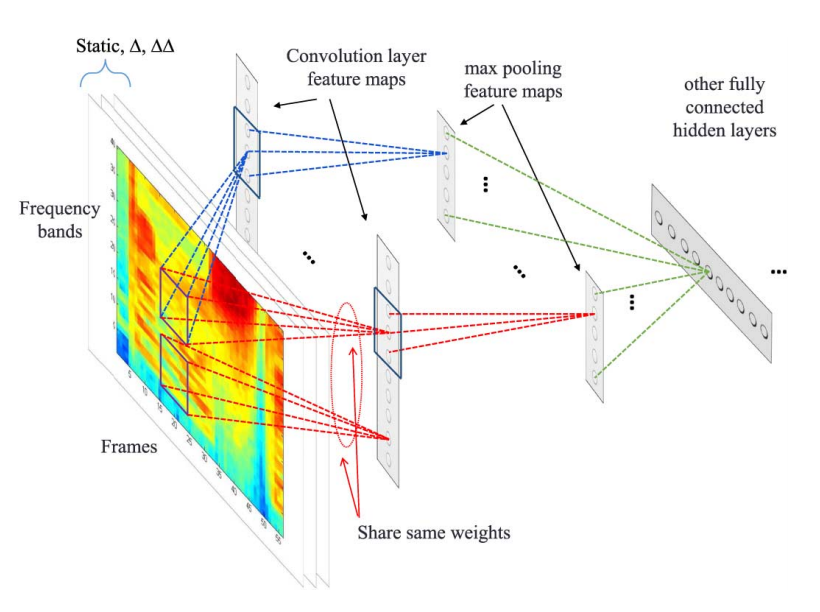
\includegraphics[width=0.7\textwidth]{cnn-audio}
	\caption{Структура CNN сети для работы с аудио сигналом.}
	\label{fig:cnn-audio}
\end{figure}

\subsubsection{Использование RNN в задаче распознавания речи}
\label{section:rnn-in-asr}
Рекуррентные нейронные сети --- один из мощных элементов глубокого обучения, позволяющий нейронным сетям работать с последовательностями данных такими как текст, аудио или видео. Отличительная особенность рекуррентных нейронных сетей --- наличие внутренней памяти, которая позволяет сети запоминать результаты обработки прошлых элементов последовательности и использовать их при анализе новых элементов. Таким образом у RNN два входа: текущий элемент и результат обработки предыдущих элементов. Структура базовой RNN сети представлена на рисунке \ref{fig:rnn-basic-structure}.

\begin{figure}[h]
	\centering
	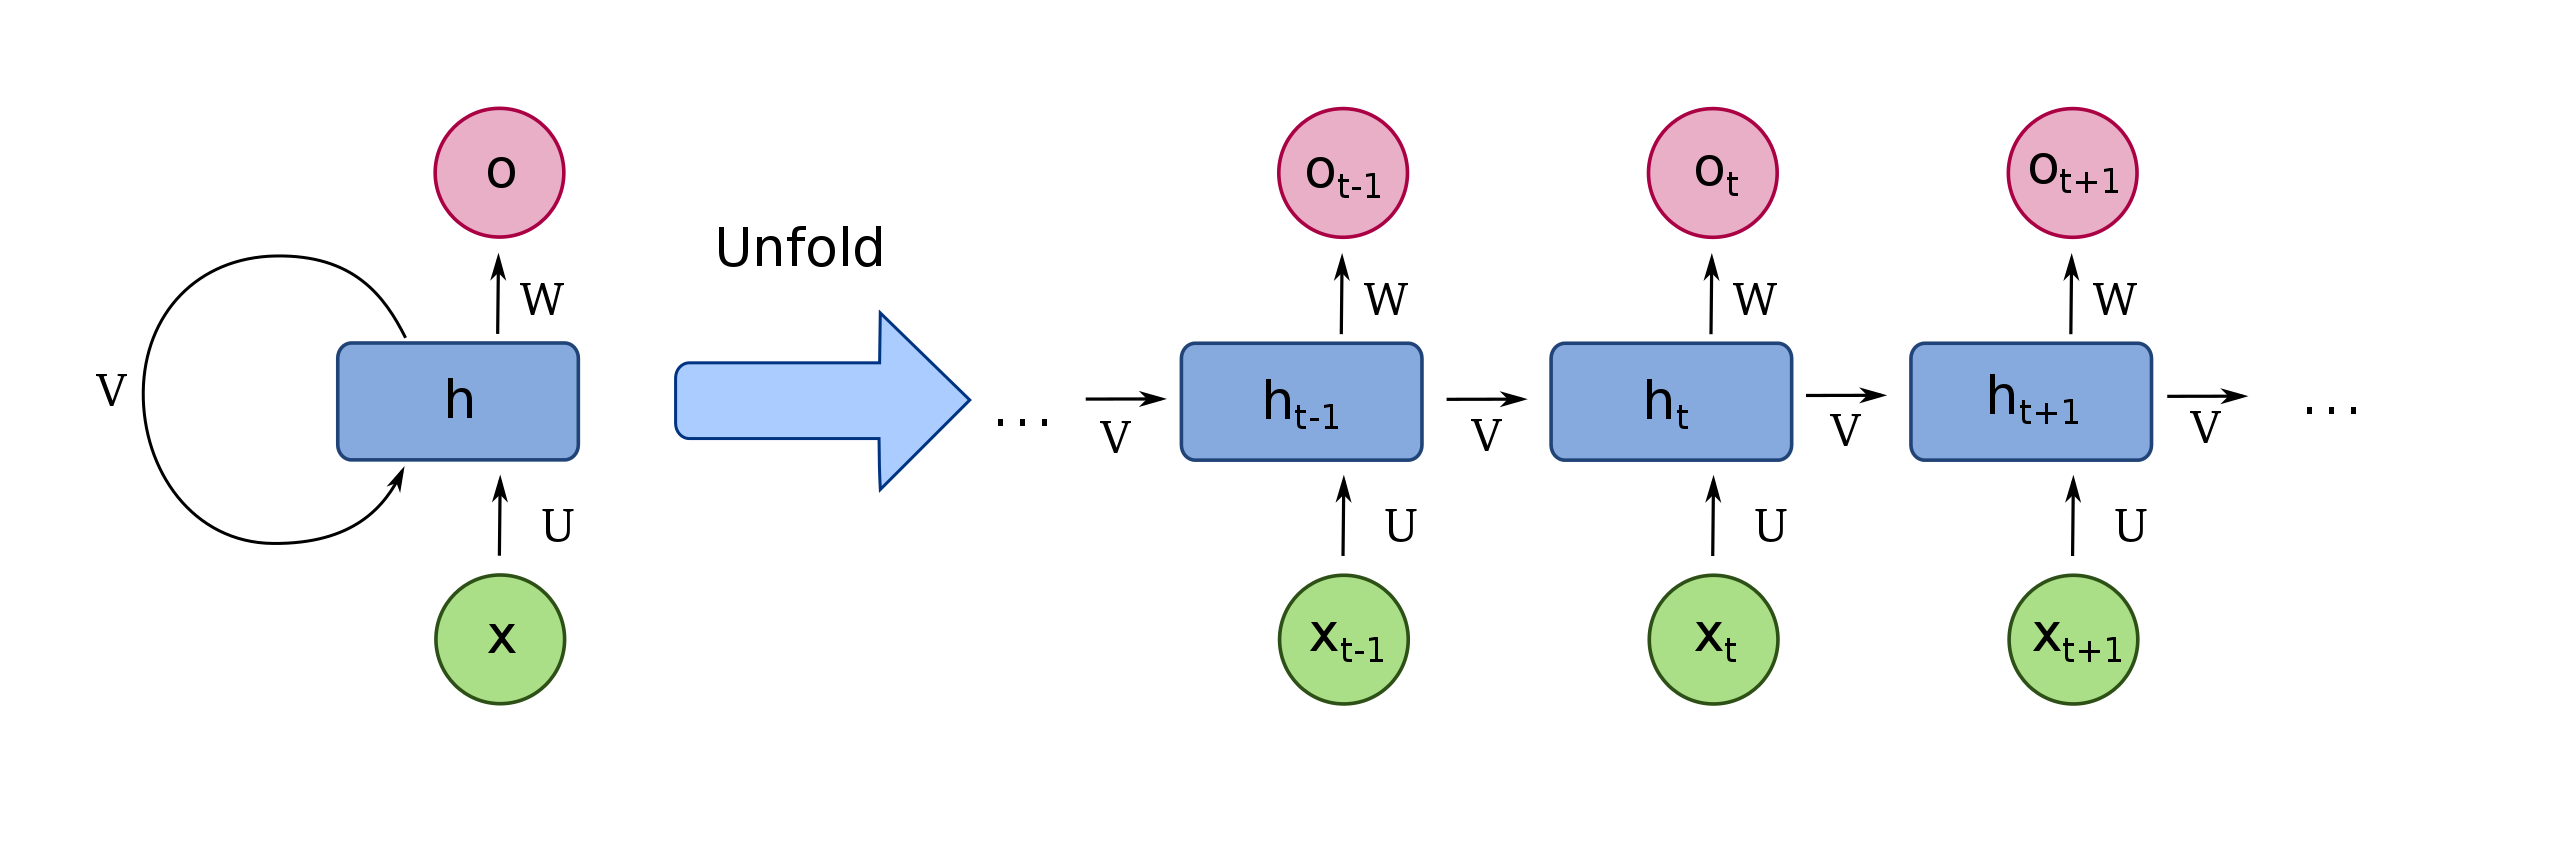
\includegraphics[width=0.7\textwidth]{rnn-basic-structure}
	\caption{Структура базовой RNN сети.}
	\label{fig:rnn-basic-structure}
\end{figure}

В своем базовом варианте рекуррентные сети страдают от проблем затухающих и возрастающих градиентов при работе с длинными последовательностями.

Эта проблема была решена внедрением \emph{Long Short-Term Memory} (LSTM)\cite{hochreiter1997long} --- расширения RNN сетей, которое модифицирует процесс работы с памятью. LSTM предоставляет возможность читать, записывать и удалять информацию из своей памяти. Каждый компонент решает, сохранять ли поступающую информацию в зависимости от того, насколько важной она является. Обзор структуры LSTM компонента приводится на рисунке \ref{fig:lstm-cell}.

\begin{figure}[h]
	\centering
	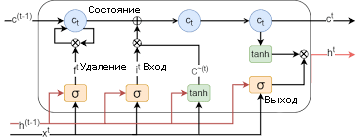
\includegraphics[width=0.7\textwidth]{lstm-cell}
	\caption{Структура одного компонента LSTM.}
	\label{fig:lstm-cell}
\end{figure}

Двунаправленные LSTM (BLSTM) сети\cite{graves2013speech, huang2015bidirectional} в каждый момент времени имеют доступ как к прошлым данным, так и к будущим, что позволяет им гораздо лучше анализировать контекст и ориентироваться во входной последовательности.

\subsubsection{Применение CTC в автоматическом распознавании речи}
Алгоритм \emph{Connectionist Temporal Classification} был впервые опубликован в 2006 году\cite{graves2006connectionist} и с тех пор широко применяется при обучении глубоких нейронных сетей в распознавании речи, рукописного текста и других задачах работы с последовательностями. Мы будем рассматривать CTC в контексте распознавания речи, а именно трансформации входного аудио-сигнала в последовательность фонем.

Итак, пусть у нас есть датасет данных, содержащий набор аудио файлов и их транскрипций --- текстовых описаний. К сожалению, нам неизвестно, какие символы соответствуют каким фрагментам аудио файлов. Это значительно усложняет задачу обучения распознающей системы и делает невозможным использование ряда простых подходов, которые были бы возможны, если бы эта информация была нам известна.

Можно было бы выдвинуть предположение, что каждый символ соответствует фрагменту аудио длиной в n миллисекунд. Однако у разных людей, а иногда и в рамках одного предложения темп речи может сильно отличаться, что исключает возможность использования такого простого предположения. Для решения этой проблемы был предложен алгоритм динамической трансформации времени\cite{berndt1994using}, допускающий нелинейные изменения в темпе речи. Однако этот подход не лишен недостатков: ограниченность шаблонов, подходит только к темпу конкретного человека, сложность подготовки обучающей выборки и нестабильность работы при искажении входных данных.

Алгоритм CTC позволяет решить проблему выравнивания аудио сигнала относительно текстовых данных. Формализуем требования к алгоритму:
\begin{itemize}
	\item Необходимо найти, как соотносятся элементы входной последовательности $X = [x_1, x_2, \dots, x_T]$ аудио фрагментов к элементам выходной последовательности текстовых данных $Y = [y_1, y_2, \dots, y_U]$.
	\item Последовательности могут отличаться по длине.
	\item Изначально выравнивание между $X$ и $Y$ неизвестно.
\end{itemize}

Метод CTC для данной входной последовательности $X$ дает вероятностное распределение для всевозможных выходных последовательностей $Y$. Необходимо обучить модель так, чтобы для верного ответа условная вероятность $P(Y | X)$ была максимальной.

Нахождение оптимальной выходной последовательности происходит из уравнения
\begin{equation}
	\label{eq:ctc-result}
	\hat{Y} = \arg \max_Y P(Y | X).
\end{equation}

Ключевая идея CTC алгоритма заключается в введении пустого символа $\epsilon$, входной аудио сигнал разбивается на равные фрагменты, каждому фрагменту присваивается соответствующий символ, на последнем же этапе удаляются повторения и пустые символы $\epsilon$. Иллюстрацию такого подхода можно увидать на рисунке \ref{fig:ctc-alignment}.

\begin{figure}[h]
	\centering
	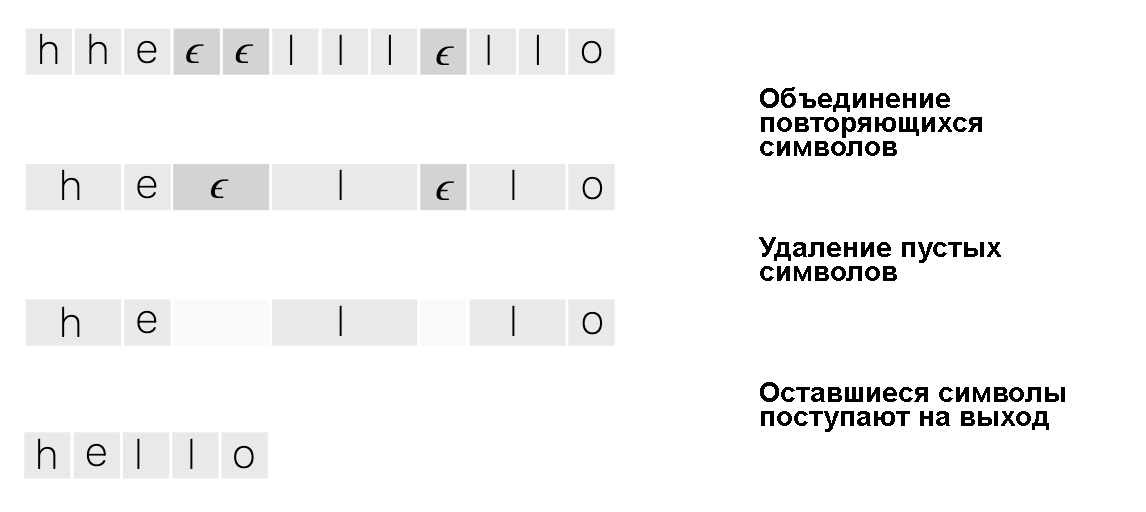
\includegraphics[width=0.7\textwidth]{ctc-alignment}
	\caption{Принцип работы выравнивания в CTC--алгоритме.}
	\label{fig:ctc-alignment}
\end{figure}

Как правило модели с использованием CTC используют рекуррентные нейронные сети, поскольку RNN учитывают контекст во входных данных. Вообще говоря можно выбирать любой алгоритм, который дает вероятностное распределение по выходным классам в зависимости от данного входа фиксированного размера. Обучение происходит с использованием элементов динамического программирования и градиентного спуска, т.е. для данного датасета $\mathcal{D}$ ставится задача минимизации:
$$\sum_{(X, Y) \in \mathcal{D}} - \log P(Y | X).$$

После обучения результат распознавания мы можем получить из уравнения \ref{eq:ctc-result} применив алгоритм beam search.

\subsubsection{Механизмы внимания в распознавании речи}
В сфере машинного обучения механизм внимания позволяет выделять более важные части входных данных и заглушать менее важные, чтобы нейронная сеть могла уделить большее внимание конкретным значимым фрагментам входных данных. Какие именно фрагменты следует считать важными зависит от контекста, но в целом определяется на этапе обучения при помощи метода градиентного спуска.

Механизм внимания может служить дополнением к системе распознавания речи. Рассмотрим, например, архитектуру Encoder--Decoder (подробнее об этой архитектуре пойдет речь в пункте \ref{section:e2e-approach}). Encoder представляет собой рекуррентную нейронную сеть (например, BLSTM) трансформирующую входную последовательность в вектор фиксированного размера $\mathbf{h}_t$, который содержит высокоуровневое представление входных данных. После того, как энкодер обработает всю входную последовательность, результат его работы, вектор $\mathbf{h}$ подается на вход декодеру. Decoder также может быть LSTM сетью, которая принимает на вход свое скрытое состояние в предыдущий момент времени и выходной символ, а в результате возвращает вероятность того, что этот символ --- корректный результат распознавания:
$$\operatorname{Decoder}(\cdot) = \operatorname{Softmax}(\operatorname{Lin}(\operatorname{LSTM}_t(\cdot))),$$
$$\mathbf{q}_t = \operatorname{LSTM}_t(\mathbf{h}_t, \mathbf{q}_{t - 1}, y_{t - 1}),$$
$$P(y_t|y_1, \dots, y_{t - 1}, X) = \operatorname{Decoder}(\mathbf{h}_t, \mathbf{q}_{t - 1}, y_{t - 1}).$$
Здесь $\mathbf{y}$ --- это результирующий вектор фонем, $\operatorname{Lin}(\cdot)$ --- линейный слой.

Такой подход имеет некоторые недостатки:
\begin{itemize}
	\item Encoder должен сжать всю входную информацию в один вектор фиксированного размера.
	\item На длинных входных последовательность точность распознавания такой системы падает.
\end{itemize}

Механизм внимания призван решить эти проблемы. Вместо того, чтобы подавать в декодер вектор $\mathbf{h}_T$, выберем наиболее релевантные фрагменты вектора $\mathbf{h}$ и отправим их на вход декодеру. Так у сети Decoder будет больше контекста и информации при генерации итогового ответа, что в целом повышает качество распознавания системы.

Мы заменяем вектор $\mathbf{h}$ на вектор $\mathbf{r}$ --- линейную комбинацию $\mathbf{h}$ и коэффициентов внимания:
$$a_{lt} = \operatorname{AttentionFunction}(\mathbf{q}_{l - 1}, \mathbf{h}_t),$$
$$\mathbf{r}_l = \sum_{t = 1}^{T} a_{lt}\mathbf{h}_t.$$
Функция $\operatorname{AttentionFunction}(\cdot)$ определяет тип внимания и отличается между разными моделями. Например, один из вариантов определения функции внимания выглядит так:
$$\operatorname{AttentionFunction}(\mathbf{q}_{l - 1}, \mathbf{h}_t) = \operatorname{Softmax}(\mathbf{g}^\top \tanh(\operatorname{Lin}(\mathbf{q}_{l - 1}) + \operatorname{LinB}(\mathbf{h}_t))).$$
Здесь $\mathbf{g}$ --- вектор, который подбирается в процессе обучения, $\operatorname{Lin}(\cdot)$ и $\operatorname{LinB}(\cdot)$ --- линейные слои без bias--вектора и с ним, коэффициенты подбираются в процессе обучения.

\subsubsection{Методы оптимизации гиперпараметров}
Гиперпараметр -- это характеристика модели, задаваемая извне и которая не может быть получена на основе данных. Так, в сверточных сетях, например, гиперпараметрами являются размер фильтров и шаг их перемещения. Значение гиперпараметров должно быть задано перед началом процесса обучения.

Задача оптимизации гиперпараметров\cite{hyperparamopt-overview} заключается в выборе набора оптимальных значений гиперпараметров для заданного алгоритма машинного обучения. Существует несколько подходов к решению этой задачи, в числе которых: сеточный поиск, случайный поиск, оптимизация на основе градиентов и другие.
Мы будем рассматривать сеточный и случайный поиск. Сеточный поиск является традиционным способом подбора оптимального решения. Его суть заключается в простом переборе всевозможных значений на заданном пространстве допустимых гиперпараметров. Обычно оценка эффективности сеточного поиска производится путем перекрестной проверки на наборе тренировочных данных, либо выполнением модели на специально выделенном валидационном наборе данных.

Поскольку пространство гиперпараметров может включать в себя действительные и неограниченные числа, перед началом подбора необходимо задать ограничения и шаг сетки.

Случайный поиск концептуально очень похож на сеточный. Основным отличием является то, что при случайном поиске перебор гиперпараметров ведется не последовательно, а на каждом шаге выбираются случайные значения\cite{hyperparamopt-random}. В случае, когда лишь небольшое число гиперпараметров оказывает значительное влияние на работу алгоритма машинного обучения, этот метод находит решение гораздо быстрее сеточного. Еще одним преимуществом случайного поиска является легкость применения параллельных вычислений.

\subsubsection{End-to-end подход в распознавании речи и анализе произношения}
\label{section:e2e-approach}
Несмотря на свою популярность, подход к автоматическому распознаванию речи с использованием скрытых марковских моделей имеет ряд недостатков:
\begin{itemize}
	\item необходимость в отдельных компонентах и обучения для звуковых моделей, произношения и языковых моделей;
	\item большой объем систем, основанных на скрытых марковских моделях, не позволяет использовать их локально на мобильных устройствах;
	\item низкая устойчивость к ошибкам в речи.
\end{itemize}

В связи с этим активное развитие получили решения с использованием глубоких нейронных сетей, предоставляющие end--to--end системы для распознавания речи\cite{graves2014towards}.

Для корректного обнаружения ошибок произношения и вывода информации по их исправлению недостаточно стандартной языковой модели. Для того, чтобы сделать распознавание ошибок возможным, была разработана расширенная распознающая сеть, которая работает совместно с традиционным решением для распознавания речи\cite{harrison2009implementation}. Тем не менее, расширенная сеть не может гарантировать, что все возможные ошибки и неточности произношения будут обнаружены. А когда распознающая система старается покрыть максимально возможное число ошибок, акустическая модель может не предоставлять необходимого уровня точности разделения между разными вариантами произношения, что ведёт к увеличению погрешности.

Чтобы преодолеть эти ограничения, были предложены другие подходы\cite{li2016mispronunciation} к распознаванию речи, для работы которых дополнительно нужна информация о буквах и соответствующих им фонемам в слове. Это позволило значительно повысить точность распознавания, однако вносит необходимость принудительного выравнивания речи относительно ожидаемых фонем. Корректность такого выравнивания напрямую влияет на точность работы алгоритма.

Мы же сфокусируемся на использовании глубоких нейронных сетей, в частности сверточных нейронных сетей и рекуррентных нейронных сетей, а также метод классификации по рейтингу (Connectionist Temporal Classification, CTC)\cite{graves2006connectionist} для создания end--to--end системы анализа произношения, которая не использует дополнительной информации о соотношении фонем с буквами в слове и не применяет методику выравнивания между разными лингвистическими единицами. CTC позволяет обучать рекуррентные нейронные сети для работы с не размеченными аудио фрагментами напрямую\cite{graves2014towards, audhkhasi2017direct}. Внедрение же сверточных нейронных сетей в область автоматического распознавания речи позволяет повысить точность\cite{abdel2012applying} и улучшить работу модели в условиях присутствия ошибок и неточностей в обрабатываемой речи\cite{palaz2015analysis}.

Комбинированная модель, построенная на базе CTC и механизма внимания, состоит из 4 основных компонентов:
\begin{enumerate}
	\item Энкодер, используемый одновременно и для CTC--модели, и для модели с механизмом внимания. Данный компонент преобразует набор входных звуковых фрагментов $(\mathbf{x}_1, \mathbf{x}_2, \dots, \mathbf{x}_T)$ к их высокоуровневому представлению $(\mathbf{h}_1, \mathbf{h}_2, \dots, \mathbf{h}_S)$ путём применения сверточных и рекуррентных сетей.
	\item Механизм внимания, который вычисляет вектор фиксированной длины $\mathbf{c}_l$ --- взвешенную сумму векторов $\mathbf{h}_i$, полученных из энкодера. Происходит обнаружение наиболее важных данных среди $\mathbf{h}_i$ для дальнейшего распознавания фонемы.
	\item Декодер, который по данным вектору $\mathbf{c}_l$ и предыдущим ответам $y_{1:l-1}$ обновляет своё внутреннее состояние $\mathbf{q}_l$ и вычисляет оценку следующей фонемы $y_l$.
	\item CTC--модуль вносит дополнительный вклад в оценку следующей фонемы, основанный на выравнивании между входными данными и выходной последовательности фонем $\mathbf{y}$. Данный модуль предотвращает появление сильных отклонений между ответом и входными данными при обучении, позволяет из нескольких вариантов ответа выбрать оптимальный.
\end{enumerate}

\begin{figure}[h]
	\centering
	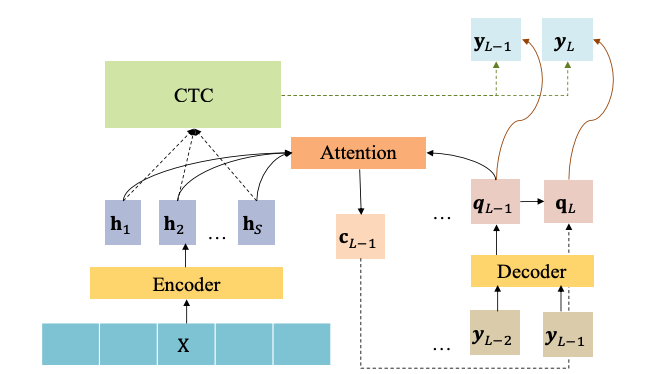
\includegraphics[width=0.7\textwidth]{ctc-att-network-architecture}
	\caption{Архитектура распознающей системы с использованием CTC и механизма внимания.}
	\label{fig:network-architecture}
\end{figure}

\begin{figure}[h]
	\centering
	\includegraphics[width=0.4\textwidth]{temp-1}
	\caption{Архитектура распознающей системы с использованием CTC и механизма внимания.}
	\label{fig:temp-1}
\end{figure}

Цель обучения такой комбинированной модели состоит в максимизации линейной комбинации двух апостериорных вероятностей, первая вероятность получается из CTC--модели, вторая --- из модели с механизмом внимания:
$$\mathcal{L} = \alpha \log P_{ctc}(\mathbf{y} | X) + (1 - \alpha)\log P_{att}(\mathbf{y} | X).$$

Здесь $\alpha$ является гиперпараметром, который определяет приоритетность каждой из моделей. На практике значение $0.5$ дает стабильные результаты.

Пусть $\mathbf{z}$ --- множество фонем вместе с пустой фонемой. Будем считать, что выходные данные в один момент времени не зависят от вывода сети в другой, то есть отсутствуют соединения между выходным слоем и самой сетью. Тогда апостериорная вероятность для CTC--модели может быть выражена следующим уравнением:
$$P_{ctc}(\mathbf{y}|X) = \sum_{\mathbf{z}} p(\mathbf{y} | \mathbf{z}, X) P(\mathbf{z} | X) \approx \sum_{\mathbf{z}} p(\mathbf{y} | \mathbf{z}) P(\mathbf{z} | X).$$

Оценка апостериорной вероятности $P(\mathbf{y}|X)$, полученная из модели с механизмом внимания может быть выражена так:
$$p(\mathbf{y}|X) = \prod_{l = 1}^{L}P(y_l | y_{1:l - 1}, X).$$
Здесь $L$ --- длина результирующего вектора $\mathbf{y}$, а вероятность $P(y_l | y_{1:l - 1}, X)$ может быть вычислена следующим образом:
$$\mathbf{h}_t = \operatorname{Encoder}(X),$$
$$a_{lt} = \operatorname{Attention}(\mathbf{q}_{l - 1}, \mathbf{h}_t),$$
$$\mathbf{r}_l = \sum_{t = 1}^{T} a_{lt}\mathbf{h}_t,$$
$$P(y_l | y_{1:l - 1}, X) = \operatorname{Decoder}(\mathbf{r}_l, \mathbf{q}_{l - 1}, y_{l-1}).$$
В качестве сети--энкодера обычно используются двунаправленные LSTM--сети\cite{graves2013hybrid}. Для сети--декодера используются однонаправленные LSTM--сети.

Ответом на поставленную задачу распознавания является наиболее вероятная последовательность фонем $\hat{\mathbf{y}}$ для заданных входных данных $X$:
$$\hat{\mathbf{y}} = \arg \max_{\mathbf{y} \in \mathbf{z}} \log P(\mathbf{y} | X).$$

Как вычисляется вероятность $P(\mathbf{y}| X)$ мы рассмотрели ранее, а поиск $\hat{\mathbf{y}}$ производится с помощью алгоритма beam search\cite{wiki:Beam_search, watanabe2017hybrid}.

Ошибки произношения можно условно разделить на две категории: явные, в которых происходит замена фонемы на другую, появление лишних или удаление некоторых фонем, и неявные, в которых фонема была произнесена с отклонениями, например, в сторону родного языка. Явные ошибки произношения покрываются построенной нами моделью. 

Для корректной обработки ошибок, связанных с модификацией звуков, введем множество так называемых анти--фонем\cite{yan2020end}. До этого в множество $\mathbf{z}$ мы включали все фонемы языка и пустой звук. Теперь же для каждой фонемы мы вводим её модифицированную версию, отметив её специальным префиксом \#. Таким образом модель распознавания будет работать с новым множеством возможных ответов:
$$\hat{\mathbf{z}} = \mathbf{z} \cup \mathbf{z}_{anti}.$$
Благодаря расширению множества мы можем разделять ошибки произношения, связанные с удалением, пропуском или заменой фонемы, и ошибки, в которых происходит искажение эталонного звука. Таким образом становится возможным корректно обрабатывать целый класс возможных неточностей произношения и в случае ошибочных модификаций звуков связывать их с соответствующей фонемой из множества $\mathbf{z}_{anti}$.

Обучение полученной системы можно произвести на датасетах TIMIT\cite{garofolo1993darpa} и L2-ARCTIC\cite{zhao2018l2}, которые содержат данные как корректных вариантов произношения, выполненных носителями языка, так и речь студентов, содержащую неточности и ошибки.

\subsubsection{Вывод по главе}
В этой главе было представлено несколько подходов к автоматическому распознаванию и анализу ошибок произношения, а также связанные с ними технологии: скрытые марковские модели, сверточные и рекуррентные нейронные сети, CTC--модели, механизмы внимания и, наконец, end--to--end система, сочетающая в себе все эти компоненты. Система, построенная на основе синтеза CTC--модели с механизмом внимания, значительно упрощает процесс реализации и обучения, так как не требует лингвистических ресурсов, таких как словарь фонем, языковой модели или морфологического анализатора, на основе которых ранее работали стандартные алгоритмы. Несколько предложенных модификаций позволяет использовать модель, направленную прежде всего на распознавание речи, для решения задачи поиска и анализа ошибок произношения. В последующих разделах будет представлено практическое использование данных алгоритмов в качестве компонента мобильного приложения для автоматической проверки речи студента.
